El propósito de un octavador es proporcionar una señal una octava inferior a la señal introducida en tiempo real. Para ello, debe haber un algoritmo que implemente una transformación al dominio de la frecuencia analizando cada muestra, posteriormente, se reducirá esa frecuencia entrante a la mitad para realizar la transformada inversa y obtener la señal octavada. 

Durante todo el siglo XX se han ido desarrollando diferentes técnicas de tratamiento y codificación para la voz, conforme iba la tecnología en aumento. La consecuencia de ello es la aparición de diversos algoritmos que permiten este tipo de operaciones con una carga computacional relativamente baja. Para este proyecto, se realizará una aproximación de \emph{"Vocoder de fase"}\footnote{Del inglés "phase vocoder"} que se podrá aplicar tanto a la voz como a cualquier instrumento, como se verá más adelante.

\section{Vocoder}
Un \emph{Vocoder}\footnote{Del inglés voice (voz) junto a encoder (codificador)} es generalemente cualquier aparato que analiza y/o sintetiza la voz humana para lograr algún objetivo concreto, como compresión de datos, multiplexación o encriptación en la mayoría de los casos.

El Vocoder de canal\footnote{Del inglés "channel vocoder"}, desarrollado por los famosos \emph{Bell Labs} en 1928, utilizaba varios filtros multibanda seguidos por detectores de envolvente cuyas señales de control se transmitían al decodificador del receptor. Estas señales de control son mucho más lentas que la señal original a transmitir, por lo que se puede reducir el ancho de banda permitiendo a un mismo medio de transmisión soportar un mayor número de canales, ya sea por radio o cable. Finalmente, el decodificador amplifica estas señales de control y las introduce en los filtros correspondientes a cada banda para poder sintetizar de nuevo la señal original. Además de las ventajas sobre el ancho de banda, también se ayuda a proteger la señal para que no se pueda interceptar. Encriptando las señales de control y modificando los parámetros de los filtros, se puede hacer muy difícil su correcta reinterpretación si no se sincronizan el codificador y el decodificador. Esto popularizó su uso durante la Segunda Guerra Mundial en el bando aliado patentándose diversos diseños.

El concepto se ha mantenido contante durante todo el siglo hasta nuestros días, donde podemos ver implementaciones modernas de la misma idea, por lo que se ha desarrollado una estandarización. La voz humana posee un rango de frecuencias de entre 200 y 3400 Hz típicamente, por lo que se optó por una frecuencia de muestreo de 8 kHz. Es común que se utilice una codificación con 16 bit por muestra por analogía con el estandar CD, pero con utilizar al menos 12 la mayoría de los receptores será capaz reproducir la señal con una fidelidad razonable. Citando un ejemplo, los codificadores según la norma ITU G.729, que son utilizados en telefonía comercial, tienen una buenísima calidad con una tasa binaria de 8 kbps. Actualmente también se utilizan para desarrollar tecnologías relacionadas con la lingüistica, la física y la neurociencia.

\subsection{Vocoder en la música}
Paralelamente a su utilización en comunicaciones, el vocoder se comenzó a popularizar durante la década de los 70 como método de síntesis. Cabe mencionar, que durante esta década, surge un gran interés en los músicos por experimentar con diferentes timbres y sonidos en instrumentos conocidos o experimentales. Para aplicaciones musicales, se utiliza una frecuencia portadora proveniente de un instrumento en lugar de extraer la frecuencia fundamental del sonido que se esta grabando. El resultado es una deformación del sonido capturado que, por estar afinado en una nota adecuada, produce un resultado agradable al oído. Fue el primer fabricante de sintetizadores y pionero de la música electrónica, Robert Moog, el que desarrollo un prototipo llamado \emph{Farad} en 1968 pero no fue hasta 1970 cuando unieron el funcionamiento de esta máquina con el sintetizador modular \emph{Moog} que había lanzado previamente al mercado. Quedaba ya conformada la esencia de utilizar la señal proveniente de un micrófono como moduladora y la proveniente de sintetizador como portadora para modularla. Algunos ejemplos tempranos de músicos reconocidos  que utilizaron estos dispositivos fueron Phil Collins, Mike Oldfield, Stevie Wonder, Herbie Hancock o Michael Jackson.

\begin{figure}
\begin{center}
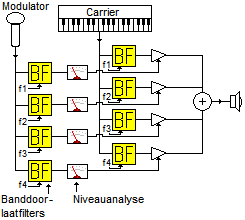
\includegraphics[width=7cm]{img/music_vocoder.png}
\caption{Esquema del funcionamiento de un vocoder musical}
\end{center}
\end{figure}

Estos vocoder proporcionaban sonidos a los que el público estaba poco acostumbrado pero que realmente no mantenían una fidelidad tímbrica respecto el sonido que captaban. Por ello se empezaron a utilizar los vocoder de fase los cuales permiten llevar a cabo expansión o compresión en el tiempo y \emph{Pitch Shifting}, es decir, modificar la altura musical del sonido o afinación sin cambiar la forma de onda que proporciona el timbre característico.

El método para hacerlo es el siguiente. En primer lugar se lleva a cabo una transformada mediante STFT (Short Time Fourier Transform) para posteriormente modificar la afinación mediante sub y sobremuestro. Este proceso hace que el audio resultante no resulte reconocible, por lo que es necesario ajustar el valor de la fase de cada muestra para mantener la coherencia entre ellas, de ahí el nombre de vocoder de fase. Una vez calculadas las muestras, se transforman de vuelta al dominio del tiempo, donde se rellena con ceros para obtener la misma duración que la señal entrante. A continuación se explican en detalle estas etapas.

\section{Transformación a frecuencia: STFT}

Una STFT se usa para determinar el módulo y fase de muestras próximas de una señal mientras cambia con el tiempo, haciéndola muy adecuada para aplicaciones en tiempo real. Para ello, se divide la señal en segmentos más cortos de la misma longitud y se calcula la transformada de Fourier de cada uno de ellos por separado. El método para calcular la transformada es indiferente pero al priorizar una baja latencia conviene decantarse por el algoritmo de la Transformada Rápida de Fourier o FFT, no obstante, se explica con mayor detalle posteriormente.

La división de las muestras se realiza por dos razones: en primer lugar nos permite acotar el número de muestras para realizar la transformada propiamente dicha (limitado por el Hardware) y en segundo lugar favorece una reconstrucción suave de la señal si se lleva a cabo de una forma adecuada.

\subsection{Solapamiento y enventanado}

Dividir la señal entrante en sucesivas tramas es un proceso sencillo, únicamente se almacenan las muestras en una memoria para introducirlas posteriormente en el módulo que realiza la FFT. Sin embargo, el proceso de reconstrucción puede llegar a ser más complicado, especialmente si se modifica la señal entre medias. Es por ello que conviene estudiar este problema con detalle teniendo en cuenta las numerosas posibilidades que existen ya desarrolladas.

La idea más intuitiva en este punto es utilizar algún tipo de \emph{solapamiento}, es decir, en lugar de empezar a construir una trama a continuación de la anterior, la empezamos a llenar antes de que se haya acabado de llenar la trama anterior, repitiendo muestras. De esta forma, las tramas están enlazadas entre ellas evitando una discontinuidad abrupt1.

Generalmente se cuantifica este proceso mediante un \emph{factor de solapamiento, fs,} expresado en tanto por ciento. Si una trama t de longitud $n = 100$ muestras tiene un solapamiento de 15\%, las primeras $n*15\% = 15$ muestras de t son idénticas a las 15 últimas de la trama anterior, t-1, y así sucesivamente.

Lógicamente, no se puede aumentar el factor de solapamiento infinitamente. A partir de un 50\% ya no resulta práctico debido a que para reconstruir la trama t se necesitan muestras de las tramas t-1 y t+1. En este caso, el beneficio de introducir este solapamiento es menor que el coste que hay que pagar: la disminución de la eficiencia del algoritmo. Idealmente realizamos el procesado sobre $n$ muestras que luego reconstruimos pero, al introducir solapamiento, solo un porcentaje de ellas, $m$, formarán parte de la señal reconstruida. En consecuencia $m < n$ siempre, lo que quiere decir que procesamos más muestras de las que utilizaremos en la reconstrucción.

La consecuencia directa de ello es un desperdicio de recursos en el procesado. Por un lado, cuanto más disminuya esta eficiencia, más aumentará la latencia, ya que habrá que esperar al cálculo de la siguiente trama para poder finalizar la construcción de la trama presente. Por otro lado, resulta mucho más complejo de cara a la temporización en su implementación. 

Como conclusión, debemos elegir un factor de solapamiento $0 < fs < 50$ para que resulte práctico. Tras un modelado en Matlab, he implementado finalmente un valor $fs = 25\%$ tal y como recomienda Ellis ~\cite{Ellis} en su implementación del vocoder de fase.


\begin{figure}[b]
\begin{center}
\label{fig:compven}
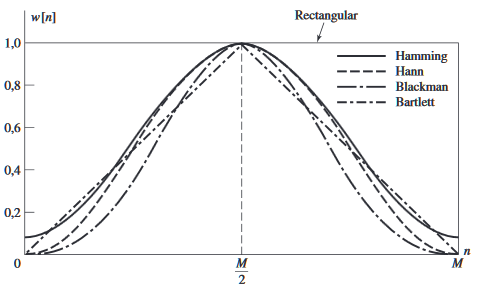
\includegraphics[width=10cm]{img/ventanas_grafica.png}
\caption{Comparativa de las ventanas más utilizadas}
\end{center}
\end{figure}

En general, estos procesos de enventanado (a excepción de la ventana rectangular) tienen la propiedad de que concentran sus transformadas de Fourier alrededor de $\omega = 0$ y además se pueden calcular fácilmente. En la figura \ref{fig:compven} se establece una comparativa entre varias de estas ventanas.

\begin{figure}
\begin{center}
\label{fig:tablaven}
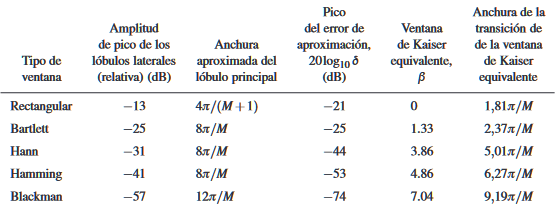
\includegraphics[width=14cm]{img/tabla_ventanas.png}
\caption{Características de las ventanas más utilizadas}
\end{center}
\end{figure}

La figura \ref{fig:tablaven} compara las ventanas desde un punto de vista más analítico. Para este caso conviene prestar  especial atención al valor de la anchura del lóbulo principal y la amplitud relativa de los lóbulos laterales. Esta última 

